\documentclass[20pt]{extarticle}
\usepackage[paperwidth=90cm,paperheight=140cm,margin=0pt]{geometry}
\usepackage{amsmath,amssymb}
\usepackage{tikz}
\usetikzlibrary{positioning,calc}
\usepackage{tcolorbox}
\tcbuselibrary{skins,breakable}
\usepackage{microtype}
\usepackage{ragged2e}
\usepackage{xcolor}
\usepackage{enumitem}
\usepackage{multicol}
\usepackage{lmodern}
\usepackage{anyfontsize}

% Redefine standard LaTeX font sizes for the poster scale
\renewcommand{\normalsize}{\fontsize{24}{30}\selectfont}
\renewcommand{\small}{\fontsize{20}{25}\selectfont}
\renewcommand{\footnotesize}{\fontsize{18}{22}\selectfont}
\renewcommand{\scriptsize}{\fontsize{16}{20}\selectfont}
\renewcommand{\tiny}{\fontsize{14}{17}\selectfont}
\renewcommand{\large}{\fontsize{28}{35}\selectfont}
\renewcommand{\Large}{\fontsize{32}{40}\selectfont}
\renewcommand{\LARGE}{\fontsize{36}{45}\selectfont}
\renewcommand{\huge}{\fontsize{40}{50}\selectfont}
\renewcommand{\Huge}{\fontsize{48}{60}\selectfont}

\AtBeginDocument{\normalsize}

\pagestyle{empty}

\definecolor{ink}{HTML}{1C1C1E} %Black
\definecolor{smoke}{HTML}{F2F2F7} %Light gray
\definecolor{rulegray}{HTML}{BBBBBB} %Gray
\definecolor{accent}{HTML}{0055AA} %Bl
\definecolor{colred}{HTML}{C0392B}
\definecolor{colgrn}{HTML}{1A6B42}
\definecolor{colblu}{HTML}{1A6B9B}
\definecolor{muted}{HTML}{777777}

\tcbset{
  sidebar/.style={enhanced,colback=white,colframe=white,
    borderline west={8pt}{0pt}{accent},
    left=20pt,right=10pt,top=10pt,bottom=10pt,boxrule=0pt,arc=0pt},
  rbar/.style={enhanced,colback=white,colframe=white,
    borderline west={8pt}{0pt}{colred},
    left=20pt,right=10pt,top=10pt,bottom=10pt,boxrule=0pt,arc=0pt},
  gbar/.style={enhanced,colback=white,colframe=white,   
    borderline west={8pt}{0pt}{colgrn},
    left=20pt,right=10pt,top=10pt,bottom=10pt,boxrule=0pt,arc=0pt},
  bbar/.style={enhanced,colback=white,colframe=white,
    borderline west={8pt}{0pt}{colblu},
    left=20pt,right=10pt,top=10pt,bottom=10pt,boxrule=0pt,arc=0pt},
  shaded/.style={enhanced,colback=smoke,colframe=smoke,
    left=25pt,right=25pt,top=18pt,bottom=18pt,boxrule=0pt,arc=12pt},
  header/.style={enhanced,colback=ink,colframe=ink,arc=0pt,boxrule=0pt,
    left=3cm,right=3cm,top=2.5cm,bottom=2.5cm},
}

\newcommand{\redd}[1]{\textcolor{colred}{\textbf{#1}}}
\newcommand{\grnd}[1]{\textcolor{colgrn}{\textbf{#1}}}
\newcommand{\mut}[1]{\textcolor{muted}{#1}}
\newcommand{\slbl}[1]{\par\noindent\begingroup\raggedright\fontsize{20}{24}\selectfont\color{muted}\MakeUppercase{#1}\par\endgroup\vspace{2mm}}
\newcommand{\stit}[1]{{\fontsize{38}{46}\selectfont\color{ink}\textbf{#1}}}
\newcommand{\shr}{{\vspace{12mm}\color{rulegray}\hrule height 2.5pt\vspace{12mm}}}

\setlist[itemize]{leftmargin=1.2em,itemsep=1pt,topsep=1pt,
  label=\textcolor{accent}{\textendash}}
\setlist[enumerate]{leftmargin=1.5em,itemsep=1pt,topsep=1pt}

\begin{document}
\color{ink}

% ── HEADER ────────────────────────────────────────────────
\noindent
\begin{tcolorbox}[header,width=\paperwidth]
    \begin{minipage}[c]{0.58\linewidth}
  {\fontsize{92}{105}\selectfont\color{white}\textbf{Subastas Shill-Proof}}\\[8mm]
  {\fontsize{34}{42}\selectfont\color{white!70!ink}
    Mathías Rolando\\[5mm]}
  {\fontsize{24}{30}\selectfont\color{white!50!ink}\itshape
    Facultad de Ciencias Exactas y Naturales\enspace·\enspace Universidad de Buenos Aires\\[3mm]}
  {\fontsize{20}{25}\selectfont\color{white!40!ink}
    Julio 2026}
\end{minipage}%
\hfill
\begin{minipage}[c]{0.8\linewidth}
  \raggedright
  {\fontsize{30}{40}\selectfont\color{white!70!ink}\itshape
    ``Qué formato de subastas le da a un vendedor \\
    \textbf{cero incentivos} para presentar ofertas falsas?''}
\end{minipage}
\end{tcolorbox}

\vspace{15mm}
% ── BODY ──────────────────────────────────────────────────
\noindent\hspace{3cm}%
\begin{minipage}[t]{47cm}

%%% LEFT %%%

\slbl{Contexto}
\stit{La práctica de las pujas falsas}

\vspace{3mm}
\begin{tcolorbox}[shaded]
\small\justifying
Las \textbf{pujas falsas} (shill bids) son ofertas ficticias que el vendedor presenta para inflar el precio final.
Los términos de Christie's permiten al subastador mover las ofertas ``hacia adelante o hacia atrás en la forma que él decida''.
En eBay, se estima que aproximadamente el \textbf{10\% de los postores en eBay Motors} son falsos, a pesar de una prohibición explícita.

\medskip
La teoría estándar esquiva esto asumiendo controles externos al mecanismo.
\emph{Este artículo se pregunta: ¿puede el propio formato de subasta eliminar el incentivo de realizar pujas falsas?}
\end{tcolorbox}

\shr

\stit{Modelo}

\vspace{3mm}
{\small\justifying
Subasta en forma extensa de un único objeto, $N$ postores potenciales, valores $\theta_i\!\sim\! F$ i.i.d.
\textbf{Postores falsos} (shills) $S$: valor privado cero, utilidad $=$ ingresos del vendedor $\sum_{j\in R}t_j$, observan todas las acciones.
\textbf{Postores reales} $R$: utilidad cuasi-lineal $x_i\theta_i - t_i$.}

\vspace{8mm}
\noindent
\begin{minipage}[t]{0.47\linewidth}
\begin{tcolorbox}[rbar]
{\small\textbf{Fuertemente Shill-Proof}}\\[6pt]
{\footnotesize Estrategia dominante ex-post de no pujar falsamente: no es rentable incluso con \textbf{conocimiento total} de los valores de los demás.}
\end{tcolorbox}
\end{minipage}\hfill
\begin{minipage}[t]{0.47\linewidth}
\begin{tcolorbox}[bbar]
{\small\textbf{Débilmente Shill-Proof}}\\[6pt]
{\footnotesize Existe un equilibrio donde la ganancia esperada de la puja falsa es $\leq 0$: no es rentable dada la distribución a priori (prior).}
\end{tcolorbox}
\end{minipage}

\shr

\stit{Fuertemente Shill-Proof}

\vspace{8mm}
{\small\textbf{Lema 3.1: Toda subasta fuertemente shill-proof es pay-as-bid.}}
\vspace{4mm}
\begin{tcolorbox}[sidebar]
\footnotesize Cualquier subasta SSP satisface: la transferencia del ganador depende únicamente de su propio reporte, y no del reporte de los demás, manteniendo fija su asignación:
\[
  \tilde x_\xi(\theta_\xi,\theta_{-\xi}) = \tilde x_\xi(\theta_\xi,\theta'_{-\xi})
  \;\Longrightarrow\;
  \tilde t_\xi(\theta_\xi,\theta'_{-\xi}) = \tilde t_\xi(\theta_\xi,\theta'_{-\xi}).
\]
\end{tcolorbox}

\vspace{8mm}
{\small\textbf{Teorema 3.6: La única subasta óptima y fuertemente shill-proof es la \redd{subasta holandesa}.}}
\vspace{4mm}
\begin{tcolorbox}[rbar]
\footnotesize
\emph{¿Por qué?} Cualquier oferta holandesa finaliza la subasta inmediatamente: un postor falso que puja gana el artículo, obteniendo \$0. En cualquier otro formato existe un historial donde una oferta falsa eleva la reserva efectiva o infla la competencia percibida sin finalizar la subasta, haciendo que las pujas falsas sean rentables.
\end{tcolorbox}

\vspace{8mm}
{\small\justifying\textbf{Estructura de información (Proposición 3.3).}\enspace
La subasta de primer precio es SSP solo bajo una estructura estática (a sobre cerrado). Cualquier filtración de información entre postores rompe la propiedad SSP.}

\end{minipage}%
\hspace{2cm}%
\begin{minipage}[t]{35cm}

%%% RIGHT %%%

\stit{Shill-proofness débil}

\slbl{El trilema}
\begin{tcolorbox}[shaded]
\footnotesize\textbf{Teorema 4.3.}\enspace Ninguna subasta ordenada puede ser simultáneamente de acción única, levemente compatible con incentivos (IC) ex-post y débilmente shill-proof.

\smallskip\emph{Bosquejo de la demostración:} WSP obliga a que la transferencia del ganador sea independiente de los reportes de los postores posteriores; la propiedad IC ex-post leve (mild EPIC) obliga a la independencia del propio reporte del ganador. La transferencia entonces solo depende de los reportes anteriores, de modo que el ganador siempre reporta $\theta^M$ para maximizar la probabilidad de ganar sin aumentar su pago, lo que rompe la regla de asignación.\hfill$\square$
\end{tcolorbox}

\vspace{6mm}

\begin{center}
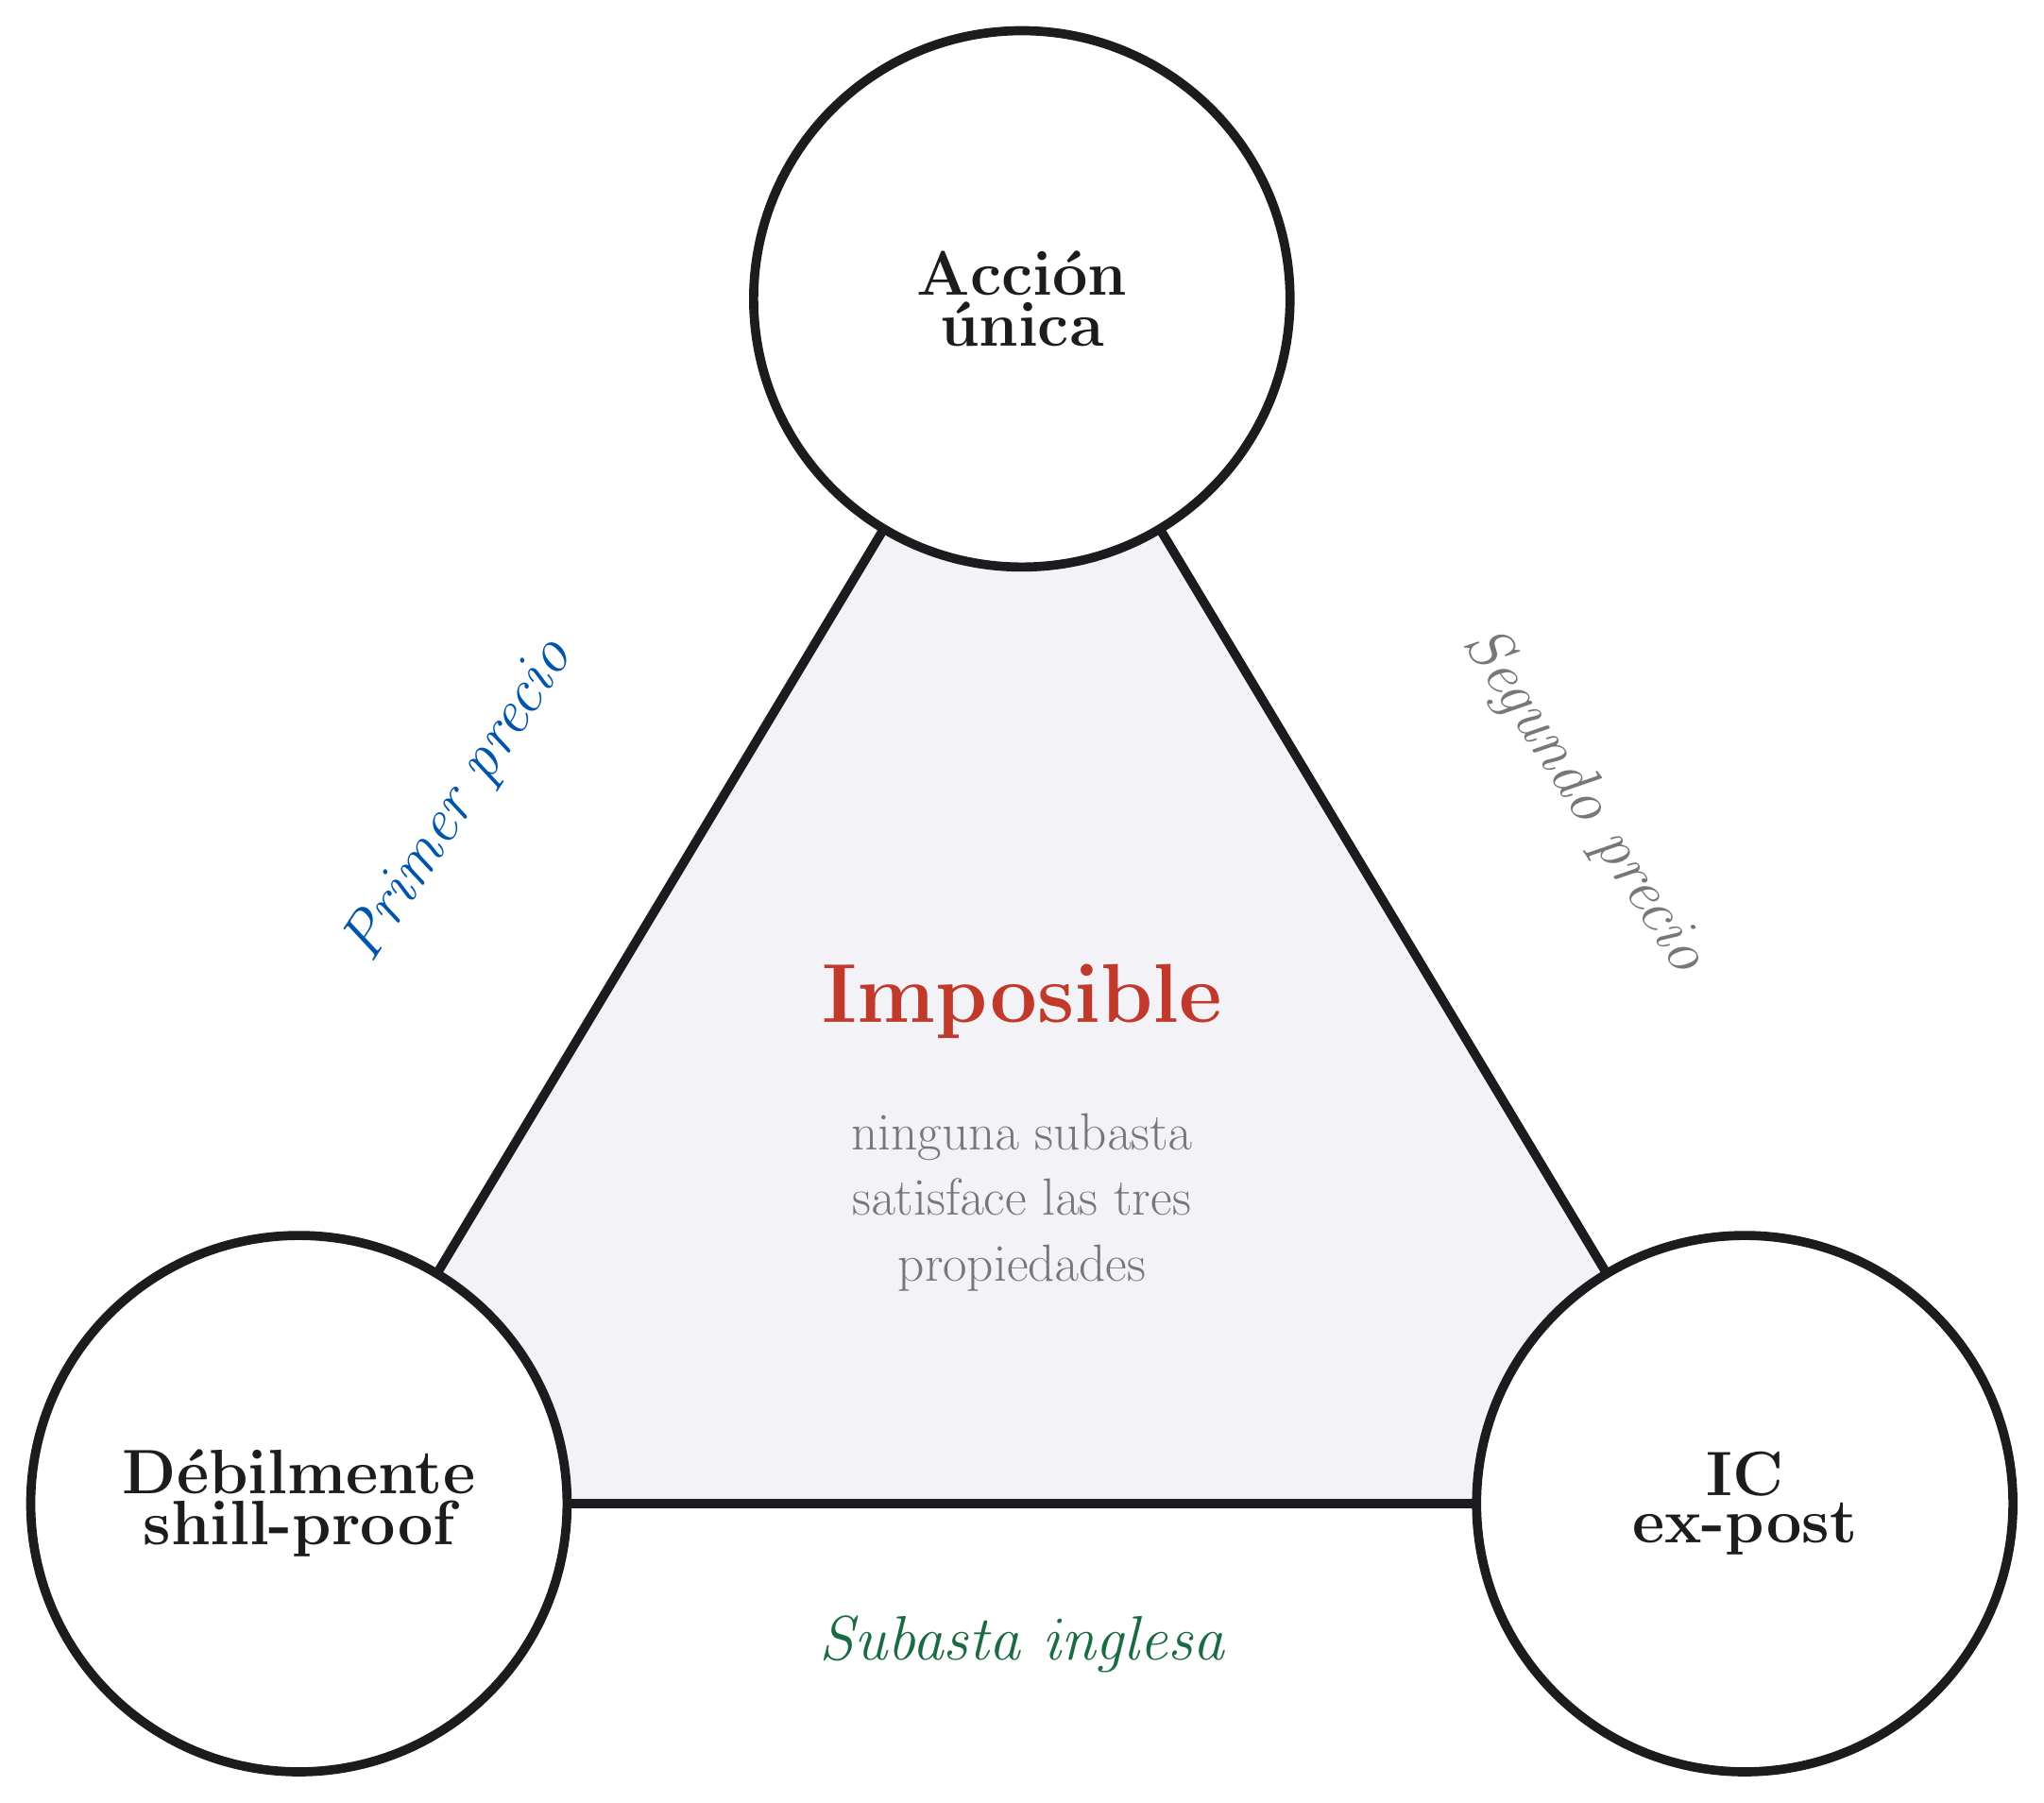
\begin{tikzpicture}[scale=2.7]
  \coordinate (A) at (0,0);
  \coordinate (B) at (7.2,0);
  \coordinate (C) at (3.6,6.0);

  % Triángulo de fondo
  \fill[smoke] (A)--(B)--(C)--cycle;
  \draw[ink,line width=3.5pt] (A)--(B)--(C)--cycle;

  % --- Etiquetas de los lados ---
  \node[font=\normalsize\itshape,text=colgrn,align=center]
    at ($(A)!0.5!(B)+(0,-0.7cm)$) {Subasta inglesa};
  \node[font=\normalsize\itshape,text=accent,align=center,rotate=57]
    at ($(A)!0.5!(C)+(-1.0cm,0.5cm)$) {Primer precio};
  \node[font=\normalsize\itshape,text=muted,align=center,rotate=-57]
    at ($(B)!0.5!(C)+(1.0cm,0.5cm)$) {Segundo precio};

  % --- Texto central "Imposible" ---
  \node[font=\Large\bfseries,text=colred] at (3.6,2.5) {\redd{Imposible}};
  \node[font=\small,text=muted,align=center]
    at (3.6,1.5) {ninguna subasta\\satisface las tres\\propiedades};

  % --- Círculos en los vértices ---
  \fill[white] (A) circle (38pt);
  \draw[ink,line width=3.5pt] (A) circle (38pt);
  \fill[white] (B) circle (38pt);
  \draw[ink,line width=3.5pt] (B) circle (38pt);
  \fill[white] (C) circle (38pt);
  \draw[ink,line width=3.5pt] (C) circle (38pt);

  % --- Etiquetas de los vértices: sin text width, usando \shortstack para centrado real línea por línea ---
  \node[font=\normalsize\bfseries,text=ink,inner sep=0pt]
    at (A) {\shortstack{Débilmente\\shill-proof}};
  \node[font=\normalsize\bfseries,text=ink,inner sep=0pt]
    at (B) {\shortstack{IC\\ex-post}};
  \node[font=\normalsize\bfseries,text=ink,inner sep=0pt]
    at (C) {\shortstack{Acción\\única}};
\end{tikzpicture}
\end{center}


\shr


\vspace{8mm}
{\small\textbf{Subastas eficientes.}}
\vspace{4mm}
\begin{tcolorbox}[gbar]
\footnotesize\textbf{Teorema 4.8.}\enspace La única subasta WSP pública, eficiente e independiente de la distribución a priori es la \grnd{subasta holandesa con reserva 0}.

\smallskip Con una reserva conocida $\theta^{\rho^*}$, cualquier subasta WSP eficiente debe ser \textbf{semi-holandesa}: debe ejecutar una fase holandesa siempre que todas las valoraciones caigan por debajo de $\theta^{\rho^*}$.

\smallskip\mut{Ejemplo del mundo real: las subastas de pescado de Honolulu-Sydney y de flores de Estambul (Hafalir et al., 2023) descienden a una fase holandesa si nadie puja al precio de apertura.}
\end{tcolorbox}

\vspace{10mm}
{\small\textbf{Más rápida que la subasta inglesa.}}

\vspace{4mm}
{\footnotesize La subasta inglesa es WSP + IC ex-post + óptima, pero consulta a cada postor hasta $M{-}\rho^*{+}1$ veces. La \textbf{subasta de cribado ascendente} (ascending-screening):
\begin{enumerate}
  \item Fase inglesa desde $\theta^{\rho^*}$ hasta el nivel de cribado $\theta^Y$.
  \item Subasta de segundo precio entre los sobrevivientes.
\end{enumerate}}

\begin{tcolorbox}[sidebar]
\footnotesize\textbf{Teorema 4.12.}\enspace Para cualquier $\varepsilon>0$, existen $F$ y $\theta^Y$ tales que la subasta de cribado ascendente es WSP, IC ex-post y óptima, mientras que
\[
  \frac{Q^{AS,Y}(F)}{Q^E(F)} \;<\; \varepsilon.
\]
\emph{Arbitrariamente más rápida que la subasta inglesa sin sacrificar la compatibilidad con incentivos (strategy-proofness).}
\end{tcolorbox}

\end{minipage}


%--------------------------------------------------------------------
\vspace{12mm}
\noindent\hspace{3cm}{\color{rulegray}\rule{84cm}{2.5pt}}
\vspace{12mm}
%--------------------------------------------------------------------


\noindent\hspace{3cm}%
\begin{minipage}[t]{47cm}

\stit{Valores afiliados e interdependientes}

\vspace{6mm}
\begin{tcolorbox}[shaded]
\footnotesize\textbf{Teorema 5.4.}\enspace La propiedad shill-proof es monótona: si una subasta es SSP (o WSP) bajo $(v,F)$, lo sigue siendo bajo $(v',F')$ siempre que
$v'\succeq_{\rm Com} v$ y $F\succeq_{\rm Aff} F'$.

\medskip\emph{Tipos más afiliados o valores más comunes hacen que la propiedad SP sea estrictamente más difícil de satisfacer.}
Todos los resultados principales se extienden a este entorno general.
\end{tcolorbox}

\end{minipage}
\hspace{2cm}%
\begin{minipage}[t]{35cm}

\stit{Extensión al concepto de credibilidad}

\vspace{6mm}
{\small\justifying Akbarpour \& Li (2020) definen la \textbf{credibilidad}: el subastador no tiene incentivos para reportar falsamente las acciones de otros postores. Nuestras nociones están relacionadas:}

\vspace{6mm}
\begin{tcolorbox}[sidebar]
\footnotesize\textbf{Teorema 6.1.}
\[
  \text{Fuertemente Shill-Proof} \;\Longrightarrow\; \text{Creíble} \;\Longrightarrow\; \text{Débilmente Shill-Proof}.
\]
Existen muchas subastas creíbles, pero solo \textbf{una} subasta óptima SSP.
El siguiente trilema generaliza el trilema de credibilidad de Akbarpour \& Li.
\end{tcolorbox}

\end{minipage}%















\vspace{20mm}
\noindent\hspace{3cm}%
\begin{minipage}{84cm}
{\color{rulegray}\hrule height 2.5pt}
\vspace{5mm}
{\footnotesize\color{muted}
  
}
\end{minipage}

\end{document}